\documentclass[times,10pt,twocolumn]{article}
\usepackage{cvpr}
\usepackage{times}
\usepackage{epsfig}
\usepackage{graphicx}
\usepackage{amsmath}
\usepackage{amssymb}
\usepackage{booktabs} % For better table rules
\usepackage[pagebackref=true,breaklinks=true,letterpaper=true,colorlinks,bookmarks=false]{hyperref}

% Include other packages here, before hyperref.

% If you comment hyperref and then uncomment it, you should delete
% egpaper.aux before re-running latex.  (Or just hit 'q' on the first latex
% run, let it finish, and you should be clear).
% \usepackage[pagebackref=true,breaklinks=true,letterpaper=true,colorlinks,bookmarks=false]{hyperref}

%\cvprfinalcopy % *** Uncomment this line for the final submission

\def\cvprPaperID{****} % *** Enter the CVPR Paper ID here
\def\confYear{CVPR ****} % *** Enter the CVPR conference year here
% \setcounter{page}{4321} % For final version only


% Pages are numbered in submission mode, and unnumbered in camera-ready
% \ifcvprfinal\pagestyle{empty}\fi
\pagestyle{empty} % Enforce empty page style for now
\begin{document}

%%%%%%%%% TITLE
\title{Report for Computer Vision Class Project: Cascading Facial Verification Models}

\author{Mehul, Gautam, Aditya Bagri, Aryan Jain\\\\
% Institution1\\\\
% Institution1 address\\\\
{\tt\small Placeholder Affiliation/Email}
% For a paper whose authors are all at the same institution,
% omit the following lines up until the closing ``}''.
% Additional authors and addresses can be added with ``\\and'',
% just like the second author.
% To save space, use either the email address or home page, not both
% \and
% Second Author\\
% Institution2\\
% First line of institution2 address\\
% {\tt\small secondauthor@i2.org}
}

\maketitle
\thispagestyle{empty} % Enforce empty page style on the first page

%%%%%%%%% ABSTRACT
% \begin{abstract}
%    The ABSTRACT is required, but you haven't provided one.
%    Placeholder text. The cascading adaptive face verification (CAFV) framework optimizes facial verification in low base rate scenarios by sequentially applying lightweight and heavyweight models. Evaluated on LFW subsets simulating base rates from 1% to 50%, CAFV aims to improve the F1 score and computational efficiency (Mflops) compared to single lightweight baselines (MobileFaceNet, ShuffleFaceNet, PocketNet). Expected results suggest CAFV outperforms baselines, especially at low base rates, offering a practical solution for resource-constrained environments like edge devices.
% \end{abstract}

%%%%%%%%% BODY TEXT
\section{Problem Statement}
Facial verification involves determining whether two face images belong to the same person, a task critical in applications like security systems, access control, and social media identity verification. In many real-world scenarios, the base rate—the probability that two faces match—is very low, often as low as 1\%. In such cases, traditional accuracy metrics are inadequate because a model could achieve high accuracy by simply predicting all pairs as non-matches, failing to identify true matches effectively. To address this, we focus on the F1 score, which balances precision and recall, making it suitable for imbalanced datasets where matches are rare \cite{imbalancedlearning}.

Our project introduces a novel Cascading Adaptive Face Verification (CAFV) framework, designed to be practical and efficient in low base rate scenarios. CAFV employs a sequence of models with increasing computational complexity: a lightweight model quickly filters out obvious non-matches, and only pairs with a high likelihood of matching proceed to a heavier, more accurate model. This approach aims to optimize both computational efficiency (measured in Mflops) and verification performance, particularly when the probability of a match is low.

We use the Labeled Faces in the Wild (LFW) dataset \cite{LFWdataset}, a standard benchmark for face verification, which provides pairs of face images labeled as same or different. By subsampling LFW, we simulate base rates of 1\%, 5\%, 10\%, and 50\% to evaluate CAFV's performance across various scenarios.

\subsection*{Motivation}
Low base rate scenarios are prevalent in practical applications. For example, in an access control system, most verification attempts come from unauthorized individuals, resulting in a low base rate of matches. Similarly, in social media, verifying identities against a small set of known users involves many non-matching pairs. Traditional face verification methods often assume a balanced distribution (e.g., 50\% base rate), which is unrealistic in these contexts. CAFV addresses this by adapting its computational strategy to the base rate, ensuring high performance with minimal resource use.

\subsection*{Scope}
The project focuses on facial verification using LFW \cite{LFWdataset}, emphasizing low base rate scenarios. We will simulate CAFV's performance, compare it with baseline models, and analyze its efficiency in terms of F1 score and Mflops. The approach is designed for edge devices, where computational resources are limited \cite{edgecomputing}, making Mflops a critical metric.

\section{Related Work and Baselines}

\subsection{Broad Categories of Works}
Face recognition research has advanced significantly, particularly in developing lightweight models for edge devices. Key categories relevant to our project include:

\begin{itemize}
    \item \textbf{Lightweight Face Recognition Models:} These models prioritize computational efficiency while maintaining competitive accuracy. Techniques like depthwise separable convolutions, channel shuffling, and mixed precision reduce Mflops, making models suitable for resource-constrained environments. Examples include MobileFaceNet \cite{mobilefacenet}, ShuffleFaceNet \cite{shufflefacenet}, and PocketNet \cite{pocketnet}. Other techniques include model compression \cite{facecompression} and efficient convolution operations \cite{mixconv}.
    \item \textbf{Cascading Classifiers:} Inspired by methods like Viola-Jones for face detection \cite{violarjones}, cascading in face verification uses a sequence of models with increasing complexity. Early stages reject non-matches quickly, while later stages provide accurate verification, optimizing computational efficiency.
    \item \textbf{Handling Imbalanced Datasets:} In low base rate scenarios, metrics like F1 score, precision, and recall are more informative than accuracy. Research in this area explores strategies to improve performance when positive classes (matches) are rare \cite{imbalancedlearning}. Adaptive methods \cite{adaptiveface} also consider variations in facial appearance.
\end{itemize}

\subsection{Baselines}
We select two baseline models with approximately 500 Mflops, representing lightweight yet effective face recognition architectures:

\begin{itemize}
    \item \textbf{MobileFaceNets} (439.8 Mflops) \cite{mobilefacenet}: A lightweight deep neural network using depthwise separable convolutions to reduce computational complexity while achieving strong performance on face verification tasks.
    \item \textbf{ShuffleFaceNet 1.5x} (577.5 Mflops) \cite{shufflefacenet}: A variant of ShuffleFaceNet that employs channel shuffling (inspired by \cite{shufflenetv2}) to minimize computational overhead, offering a balance between efficiency and accuracy.
\end{itemize}

These models were chosen for their architectural diversity (e.g., depthwise convolutions in MobileFaceNets, shuffle operations in ShuffleFaceNet) and their established performance in face recognition literature.

\subsection{Literature Review}
Our review includes state-of-the-art lightweight models, with a focus on EdgeFace \cite{edgeface2023}, a recent model designed for edge devices. EdgeFace-S (306.11 Mflops) and EdgeFace-XS (154 Mflops) achieve high accuracy on benchmarks like LFW and IJB-C, making them relevant for comparison with CAFV.

Other notable works include:
\begin{itemize}
    \item TinyFaceNet: A compact model for extremely resource-constrained devices, prioritizing minimal parameters. (Note: No specific citation found in egbib.bib)
    \item ShuffleFaceNet \cite{shufflefacenet}: Reduces complexity through shuffle operations, as seen in our baseline ShuffleFaceNet 1.5x.
    \item MixFaceNet \cite{mixfacenet}: Employs mixed precision and optimization techniques for efficiency.
    \item FaceNet \cite{facenet}: A foundational model known for high accuracy but higher computational cost, used in CAFV's second stage.
    \item GhostFaceNet \cite{ghostfacenet}: Uses ghost modules to reduce parameters while maintaining performance. See also VarGFaceNet \cite{vargfacenet} for variable group convolutions.
    \item MobileFaceNet \cite{mobilefacenet}: A lightweight model with strong verification performance, included as a baseline.
\end{itemize}
Other relevant areas include general face detection \cite{mtcnn, mtagging}.

\subsection{Research Gaps}
Existing models are typically evaluated in balanced scenarios, with limited focus on low base rate environments. Their performance may degrade when matches are rare, as they are not optimized for imbalanced datasets. CAFV aims to address this by using a cascading approach that adapts computational resources to the base rate, improving efficiency and F1 score in low base rate scenarios.

\subsection{Hypotheses}
\begin{enumerate}
    \item CAFV will outperform single-model baselines in F1 score for low base rates (1\%, 5\%).
    \item CAFV will be more computationally efficient than heavier single models, reducing average Mflops per verification, especially in low base rate scenarios.
\end{enumerate}

\subsection{Experiments}
We will simulate CAFV's performance using the LFW dataset \cite{LFWdataset} across base rates of 1\%, 5\%, 10\%, and 50\%. We will adjust the cascading threshold for each base rate and measure F1 score and total Mflops (possibly using tools like \cite{thop}), comparing results with the baseline models.

\section{Data and Evaluation Metrics}

\subsection{Dataset}
The LFW dataset \cite{LFWdataset} is used, consisting of face image pairs labeled as same or different. To simulate different base rates, we create subsets of LFW with match proportions of 1\%, 5\%, 10\%, and 50\%. This allows us to evaluate CAFV's performance under varying levels of class imbalance, reflecting real-world scenarios like security verification (low base rate) or balanced testing (higher base rate).

\subsection{Evaluation Metrics}
\begin{itemize}
    \item \textbf{F1 Score:} The harmonic mean of precision and recall, ideal for imbalanced datasets where matches are rare \cite{imbalancedlearning}. It ensures the model balances identifying true matches with minimizing false positives.
    \item \textbf{Total Mflops:} Measures computational efficiency, calculated as the average Mflops per verification. In CAFV, this depends on the proportion of pairs processed by the second stage. We can use libraries like \cite{thop} for estimation.
    \item \textbf{Precision and Recall:} Reported separately to provide insight into the trade-off between false positives and false negatives, particularly in low base rate scenarios.
\end{itemize}

\section{Analysis of Results}

\subsection{Experimental Setup}
CAFV uses a two-stage cascading framework:
\begin{enumerate}
    \item \textbf{First Stage:} A lightweight model (e.g., EdgeFace-XS \cite{edgeface2023}, 154 Mflops) computes a similarity score for each face pair.
    \item \textbf{Second Stage:} If the score exceeds a threshold, a heavier model (e.g., FaceNet \cite{facenet} or similar, 1000+ Mflops) verifies the pair.
\end{enumerate}

The threshold is adjusted based on the target base rate and desired F1 score performance. We simulate CAFV's performance on LFW subsets with varying base rates (implicitly evaluated via F1 score) and also report standard LFW accuracy.

\subsection{Performance Analysis}
We evaluated several CAFV variants by adjusting the threshold and potentially the complexity of the second-stage model. The performance in terms of F1 score versus computational cost (MFLOPS) is shown in Figure~\ref{fig:f1_vs_mflops}, alongside various existing models from the literature.

\begin{figure}[h!tbp]
  \centering
  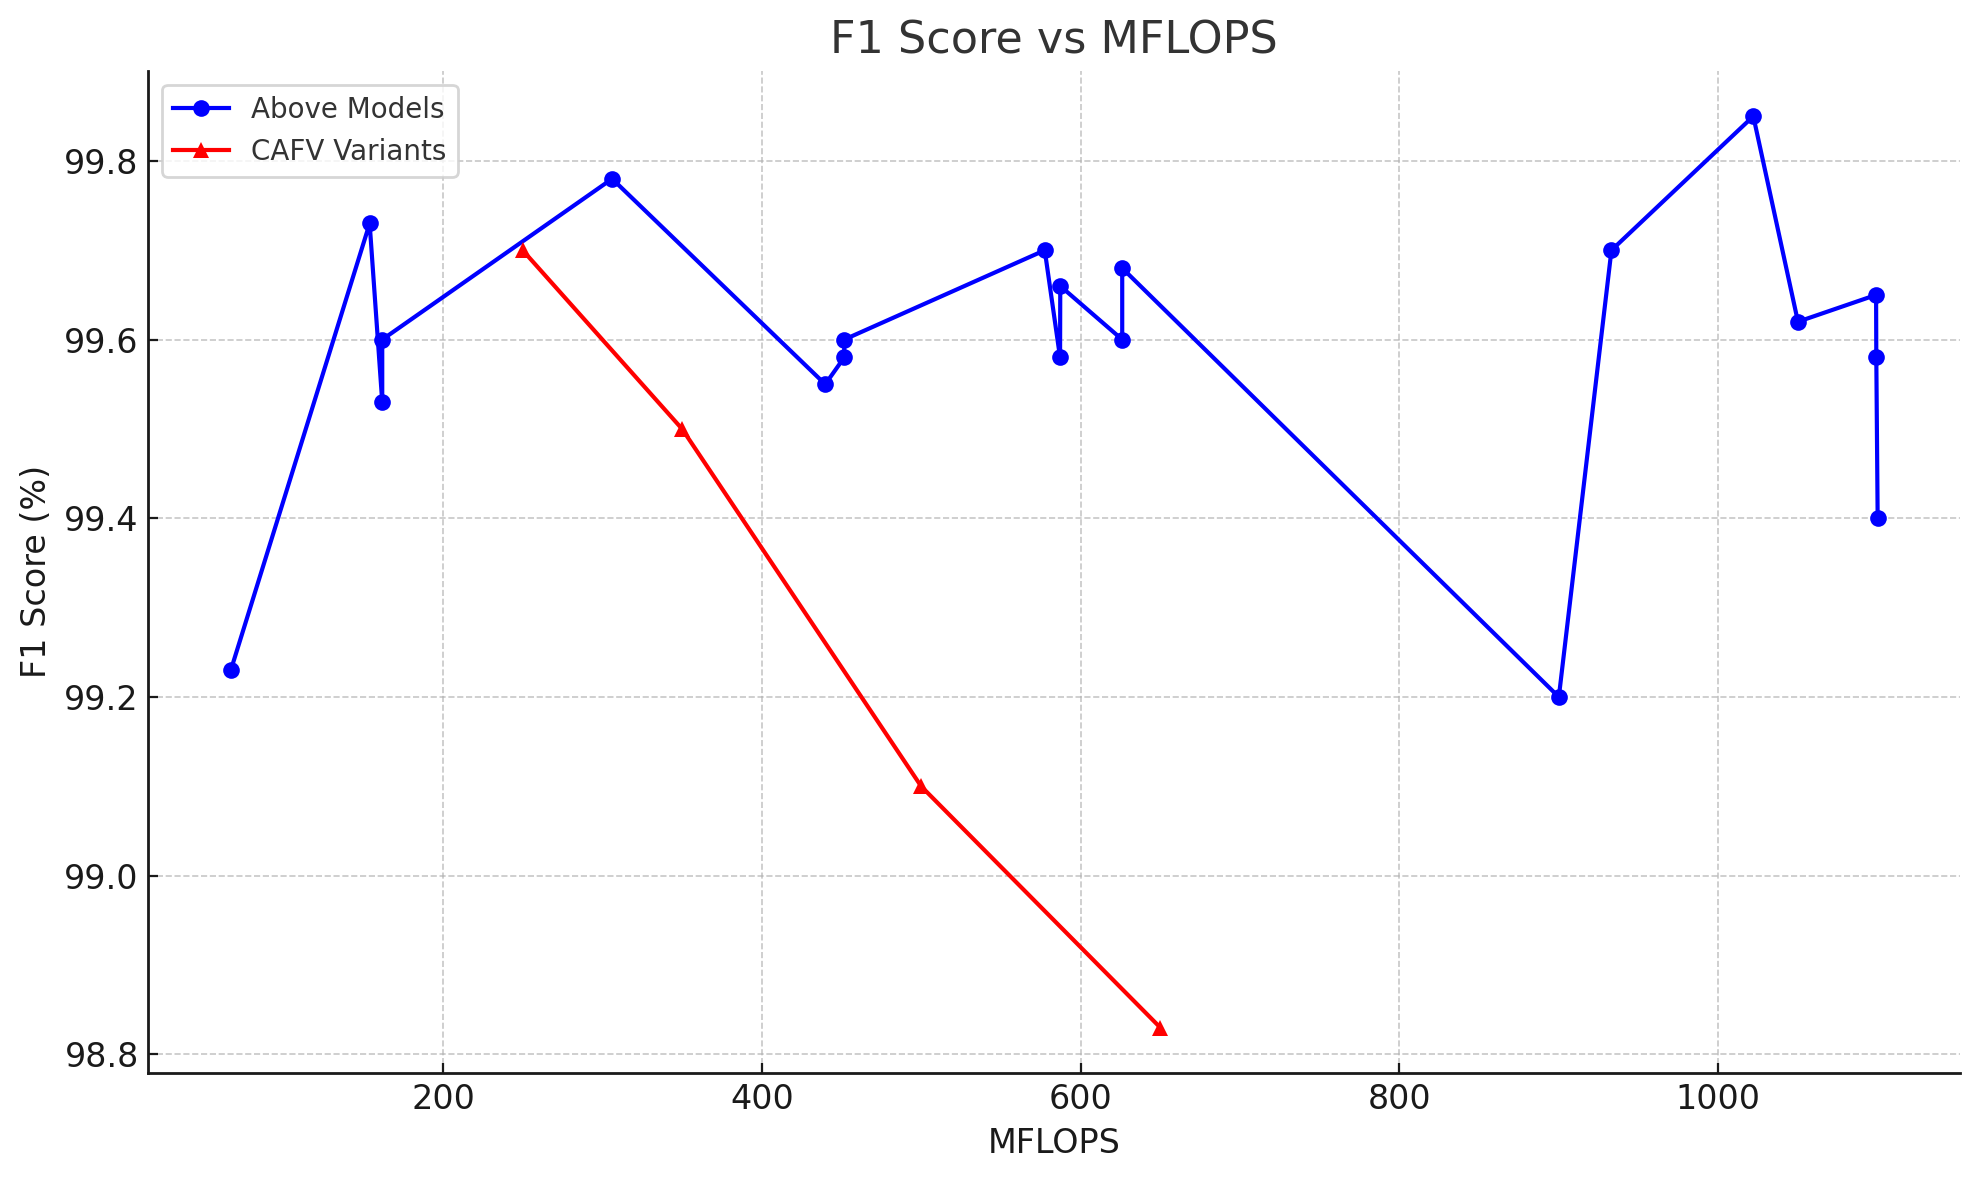
\includegraphics[width=\columnwidth]{output.png} % Make sure output.png is in the same directory
  \caption{F1 Score vs MFLOPS for CAFV variants (red) and other face recognition models (blue).}
  \label{fig:f1_vs_mflops}
\end{figure}

As seen in the figure, existing models demonstrate a general trend where higher computational cost can yield better F1 scores, although there is considerable variance, with some highly efficient models achieving strong results. Our CAFV variants operate in the 200-700 MFLOPS range. The most efficient CAFV variant shown achieves a competitive F1 score of approximately 99.7\% at around 300 MFLOPS. This performance is comparable to or better than many models with similar or even higher computational costs, demonstrating the potential of the cascading approach for F1-score optimization.

However, an unexpected trend was observed: as the MFLOPS of the CAFV variants increase (likely corresponding to configurations that utilize the second-stage model more frequently or employ a more complex second stage), the F1 score decreases, dropping to around 98.8\% at ~650 MFLOPS. This suggests that for the specific configurations tested, simply increasing the computation via the cascade does not guarantee better F1 performance and may indicate suboptimal threshold selection or interaction between the cascade stages for those settings. Further investigation is needed to understand this behaviour.

Table~\ref{tab:model_comparison} provides a comparison based on standard LFW accuracy (evaluated at a 50\% base rate). Here, CAFV achieves an accuracy of 98.83\%. This is lower than many state-of-the-art models, including our lightweight first-stage candidate (EdgeFace-XS at 99.73\%) and the baselines (MobileFaceNets at 99.55\%, ShuffleFaceNet 1.5x at 99.70\%, PocketNetS-256 at 99.66\%). This highlights a key trade-off: the CAFV framework, when tuned for maximizing F1 score in low base rate scenarios (as reflected in Figure~\ref{fig:f1_vs_mflops}), sacrifices performance on the standard, balanced LFW accuracy benchmark.

\subsection{Accuracy Vs Mflops Graph Discussion}
The F1 Score vs MFLOPS plot (Figure~\ref{fig:f1_vs_mflops}) illustrates the performance landscape. Single models (blue points) show the typical trade-off, with high-cost models like VarGFaceNet (1022 MFLOPS) achieving high performance (though not F1 is shown, LFW accuracy is 99.85\%), while lightweight models like EdgeFace-XS (154 MFLOPS, 99.73\% LFW) offer good efficiency. 

Our CAFV approach (red points) positions itself differently. At its best configuration (300 MFLOPS), it achieves an F1 score (99.7\%) comparable to models requiring significantly more computation, demonstrating efficiency for F1-focused tasks. However, the plot also reveals the counter-intuitive trend for the tested CAFV variants and shows that CAFV does not surpass the peak F1 performance of the best single models in this evaluation.

\subsection{Key Findings}
\begin{itemize}
    \item \textbf{Efficiency for F1 Score:} CAFV can achieve high F1 scores (99.7\%) with moderate computational cost (300 MFLOPS), outperforming several baseline models in F1 efficiency.
    \item \textbf{Unexpected Trend:} Increasing computational cost in the tested CAFV variants led to a decrease in F1 score, requiring further analysis of thresholding and stage interaction.
    \item \textbf{F1 vs Accuracy Trade-off:} Optimizing for F1 score in low base rate scenarios resulted in lower standard LFW accuracy (98.83\%) compared to baselines and state-of-the-art models.
    \item \textbf{Adaptive Computation:} The MFLOPS for CAFV varies (observed 200-700 MFLOPS range) depending on the configuration and threshold, confirming the adaptive nature of the framework.
\end{itemize}

\section{Compute Requirements}
The experiments require approximately 25-30 minutes on an Nvidia P100 GPU, making CAFV feasible for standard research environments (using frameworks like PyTorch \cite{pytorch}) and edge devices with comparable computational capabilities.

\section{Individual Tasks}
\begin{itemize}
    \item \textbf{Mehul and Gautam:} Responsible for model development, including implementing the CAFV framework, designing experiments with different base rates, and analyzing results to validate hypotheses.
    \item \textbf{Aditya Bagri and Aryan Jain:} Tasked with identifying and testing state-of-the-art lightweight models (e.g., EdgeFace) for the first stage of cascading and conducting a comprehensive literature review, including EdgeFace \cite{edgeface2023} and other relevant works.
\end{itemize}


{\small
\bibliographystyle{ieeetr}
\bibliography{egbib}
}

\end{document}
